\newpage
\section{236. 二叉树的最近公共祖先}
\label{leetcode:236}

\subsection{题目}

给定一个二叉搜索树, 找到该树中两个指定节点的最近公共祖先。

百度百科中最近公共祖先的定义为:``对于有根树 T 的两个结点 p、q,
最近公共祖先表示为一个结点 x,满足 x 是 p、q 的祖先且 x 的深度尽可能大
(一个节点也可以是它自己的祖先)。''

例如,给定如下二叉搜索树:  root = [6,2,8,0,4,7,9,null,null,3,5]

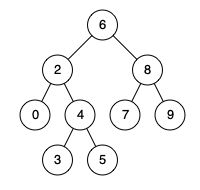
\includegraphics[width=60mm,height=60mm]{images/leetcode/binarysearchtree_improved.png}

\textbf{示例 1}:

\begin{verbatim}
  输入: root = [6,2,8,0,4,7,9,null,null,3,5], p = 2, q = 8
  输出: 6
  解释: 节点 2 和节点 8 的最近公共祖先是 6。
\end{verbatim}

\textbf{示例 2}:

\begin{verbatim}
  输入: root = [6,2,8,0,4,7,9,null,null,3,5], p = 2, q = 4
  输出: 2
  解释: 节点 2 和节点 4 的最近公共祖先是 2, 因为根据定义最近公共祖先节点可以为节点本身。
\end{verbatim}

\textbf{说明}:

\begin{enumerate}
  \item 所有节点的值都是唯一的。
  \item p、q 为不同节点且均存在于给定的二叉树中。
\end{enumerate}

\subsection{参考题解}

\subsubsection{Python}

\begin{verbatim}
# Definition for a binary tree node.
# class TreeNode:
#     def __init__(self, x):
#         self.val = x
#         self.left = None
#         self.right = None

class Solution:
  def lowestCommonAncestor(self, root: 'TreeNode', p: 'TreeNode', q: 'TreeNode') -> 'TreeNode':
    while root:
      if p.val < root.val and q.val < root.val:
        root = root.left
      elif p.val > root.val and q.val > root.val:
        root = root.right
      else:
        return root
\end{verbatim}
